Die Chatseite ist in eine Liste aus aktiven Chats und eine Warteliste aufgeteilt, siehe \ref{fig:chat_a} und \ref{fig:chat_b}. Um zwischen diesen beiden Listen zu wechseln werden Tabs eingesetzt, wie sie aus Windowsanwendungen bekannt sind. Zwischen diesen Tabs kann entweder gewechselt werden, indem ein anderes Tabfenster angetippt wird, oder der gesamte Bildschirm mit einer Geste zur Seite gewischt wird. Bei jedem Element der Chatliste ist der jeweilige Benutzername und die neueste Nachricht zu sehen, dazu wird falls vorhanden entweder ein Profilbild oder eine einfarbige Fläche mit dem Anfangsbuchstaben des Namens angezeigt. Chat Requests können jeweils durch das Schieben nach links angenommen oder nach rechts ablehnt werden, wie in den Abbildungen \ref{fig:chat_c}, bzw. \ref{fig:chat_d} zu sehen ist. Diese Mechanik wird häufig in Email-Apps zum Löschen oder Verschieben der Mails benutzt.\\ %TODO (screenshots normal, annehmen und ablehnen)
Durch Antippen eines Matches, öffnet sich der Chatverlauf, welcher in Abbildung \ref{fig:chat_e} zu sehen ist. Die Anordnung der Nachrichten innerhalb des Chatverlaufs ist wie aus anderen Messenger bereits bekannt, aber in den Stilfarben von StreamSwipe. Am oberen Bildschirmrand wird der Profilname des Matches angezeigt und rechts davon befindet sich der Button zu dessen Profilseite, auf der genauere Details über diese Person zu finden sind. Die Profilseiten werden in Kapitel \ref{sec:benutzerprofil} genauer vorgestellt. \\
Dem User wird durch das ihm bereits vorgestellte Design und der ausschließlichen Nutzung von bekannter Mechanik ein vertrautes Umfeld geboten. Wie auf jedem Screen passt sich auch hier das Farbschema automatisch an, falls in den Systemeinstellungen des Smartphones das dunkle Design gewählt wurde, wie beispielsweise in Abbildung \ref{fig:chat_f} dargestellt. Neben der Benutzerfreundlichkeit wird auch die Barrierefreiheit beachtet, indem alle Elemente, die nicht bereits aus einem Text bestehen, mit Semantiken ausgestattet werden. Zusätzlich werden keine feinmotorischen Bewegungen zur Navigation durch die Bildschirme benötigt. Bis auf die Eingabe über die Tastatur kann alles über große Flächen oder Wischmechaniken bedient werden. Im Chatverlauf wir die Standardtastatur des Systems verwendet, mit der der Benutzer bereits vertraut ist. 


\begin{figure}[H]
	\begin{subfigure}{0.33\textwidth}
	\centering
	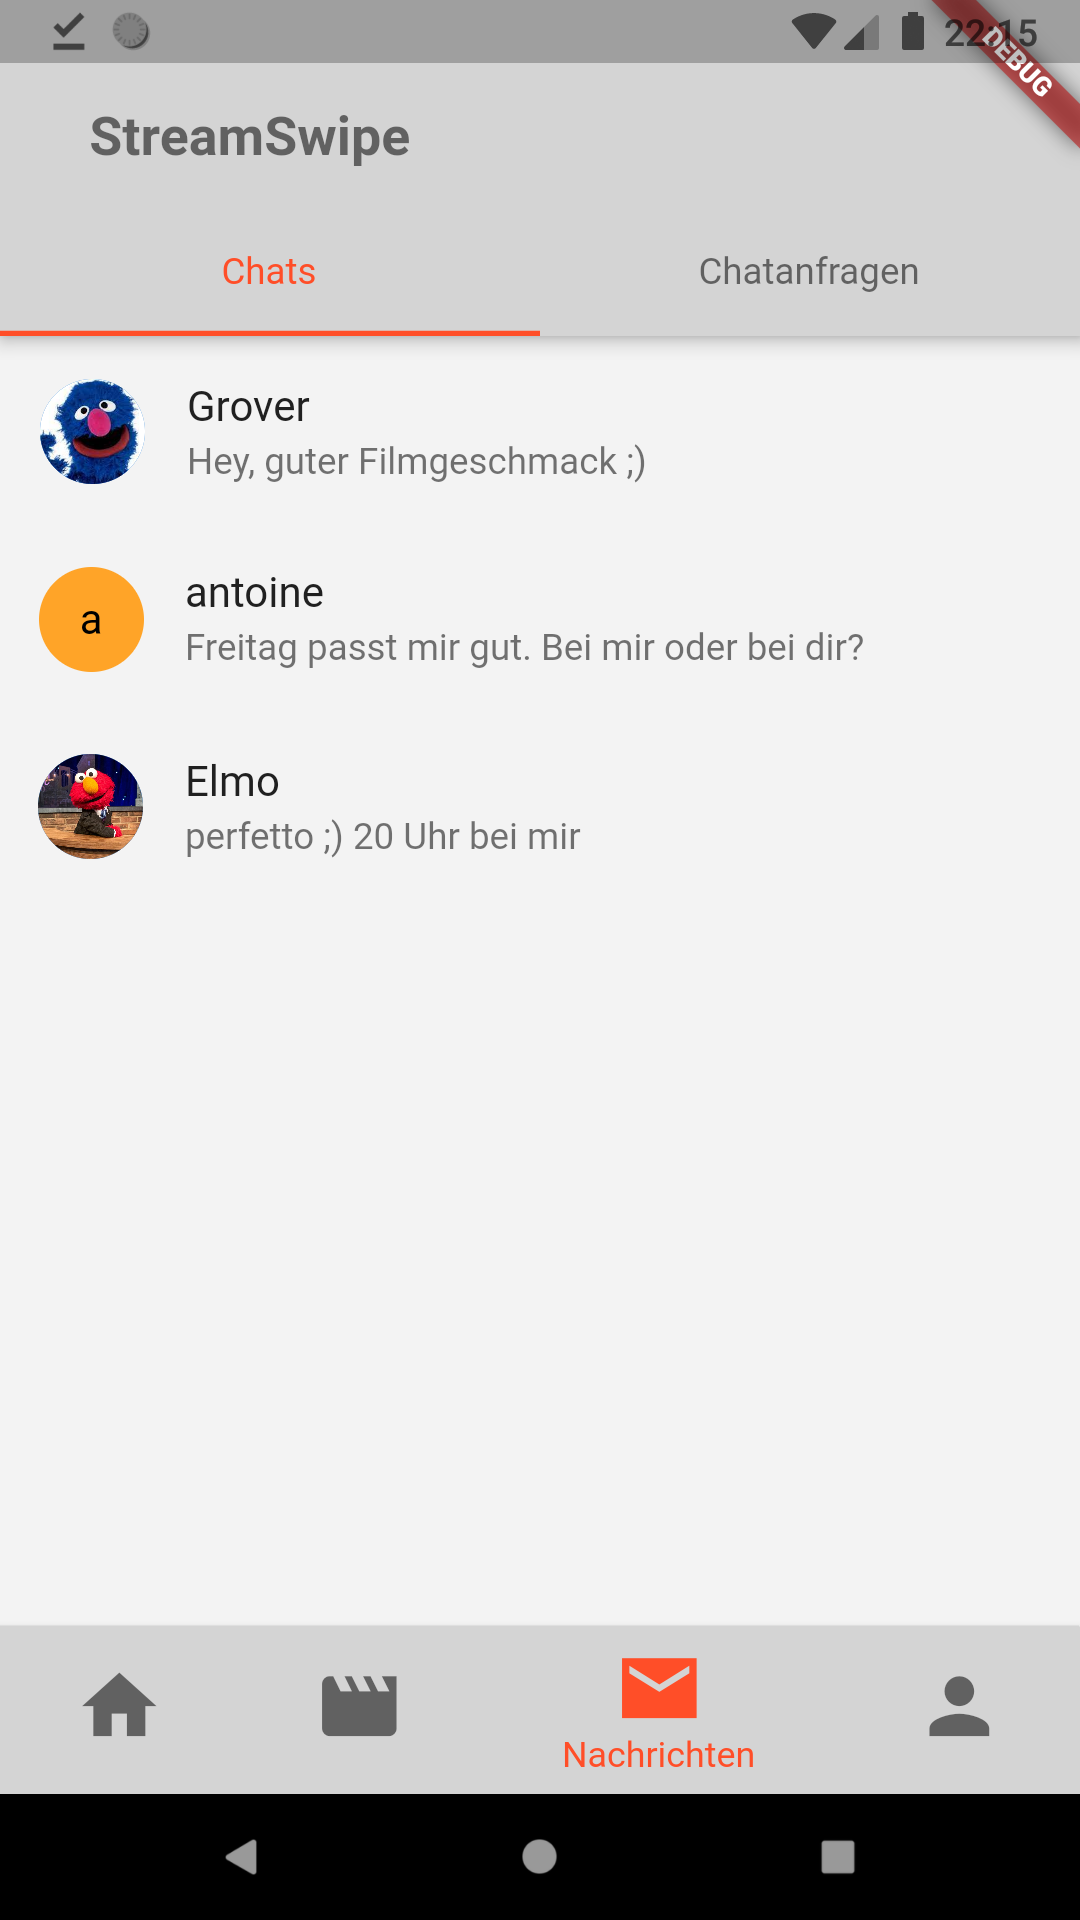
\includegraphics[scale=0.1742]{Benutzeroberfläche/images/screenshot_chat_1.png}
	\caption{}
	\label{fig:chat_a}
	\end{subfigure}
	\begin{subfigure}{0.33\textwidth}
	\centering
	
\includegraphics[scale=0.1742]{Benutzeroberfläche/images/screenshot_chat_2.png}
	\caption{}
	\label{fig:chat_b}
	\end{subfigure}
	\begin{subfigure}{0.33\textwidth}
	\centering
	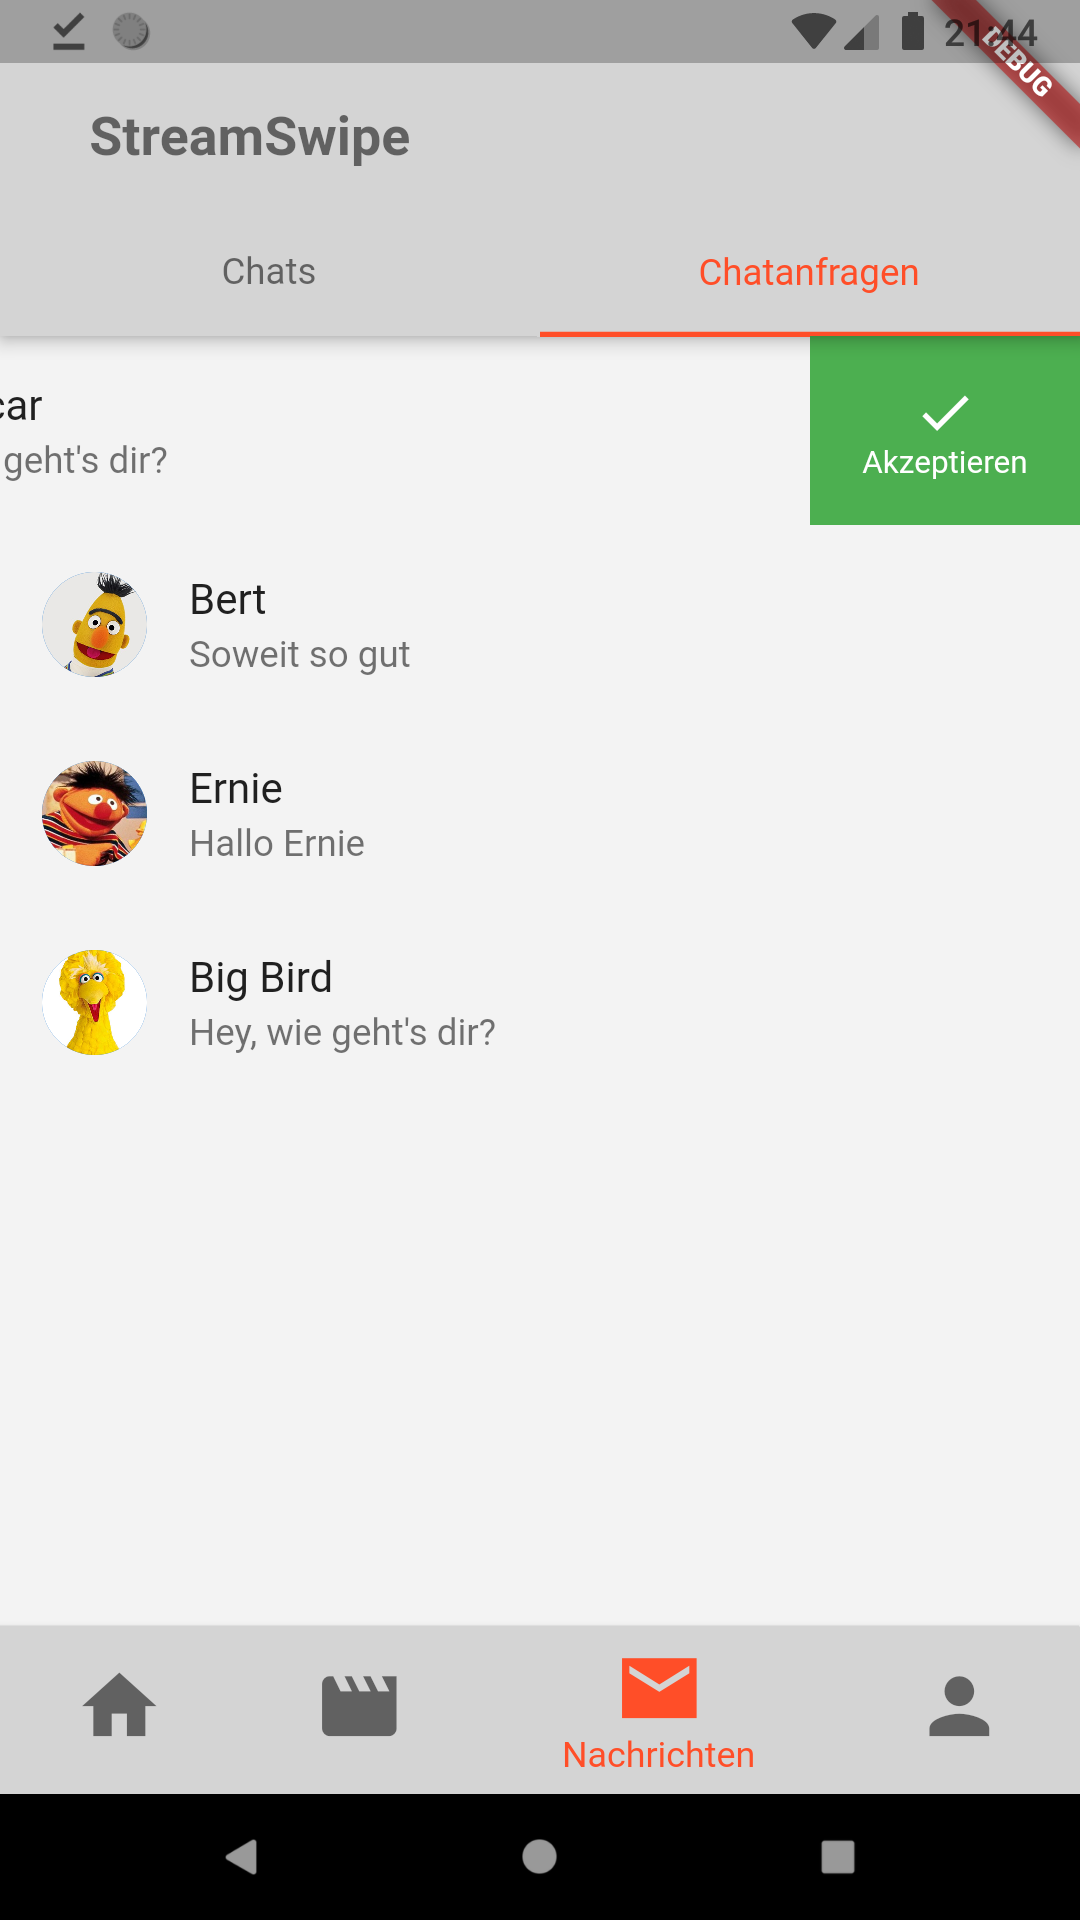
\includegraphics[scale=0.1742]{Benutzeroberfläche/images/screenshot_chat_3.png}
	\caption{}
	\label{fig:chat_c}
	\end{subfigure}\\ \vspace{1cm}	
	
	\begin{subfigure}{0.33\textwidth}
	\centering
	
\includegraphics[scale=0.1741]{Benutzeroberfläche/images/screenshot_chat_4.png}
	\caption{}
	\label{fig:chat_d}
	\end{subfigure}
	\begin{subfigure}{0.33\textwidth}
	\centering
	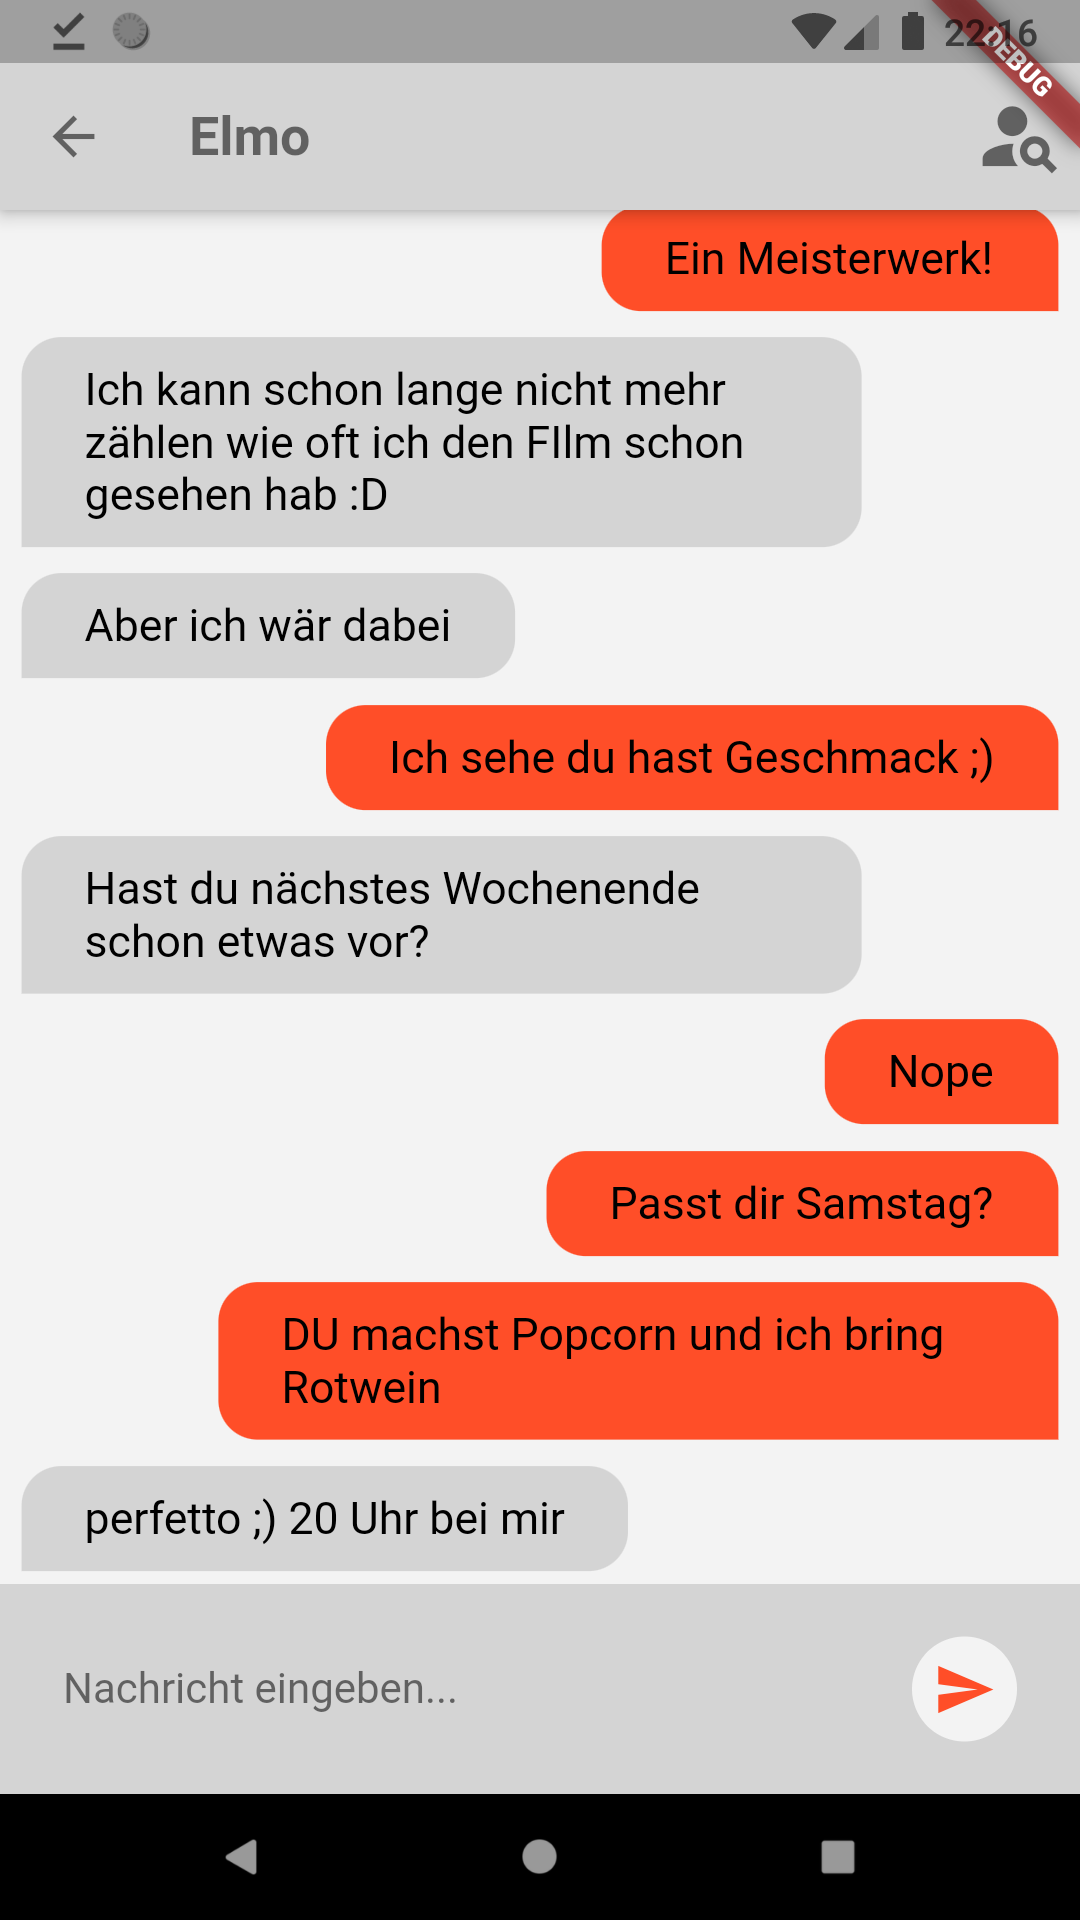
\includegraphics[scale=0.13]{Benutzeroberfläche/images/screenshot_chat_5.png}
	\caption{}
	\label{fig:chat_e}
	\end{subfigure}
	\begin{subfigure}{0.33\textwidth}
	\centering
	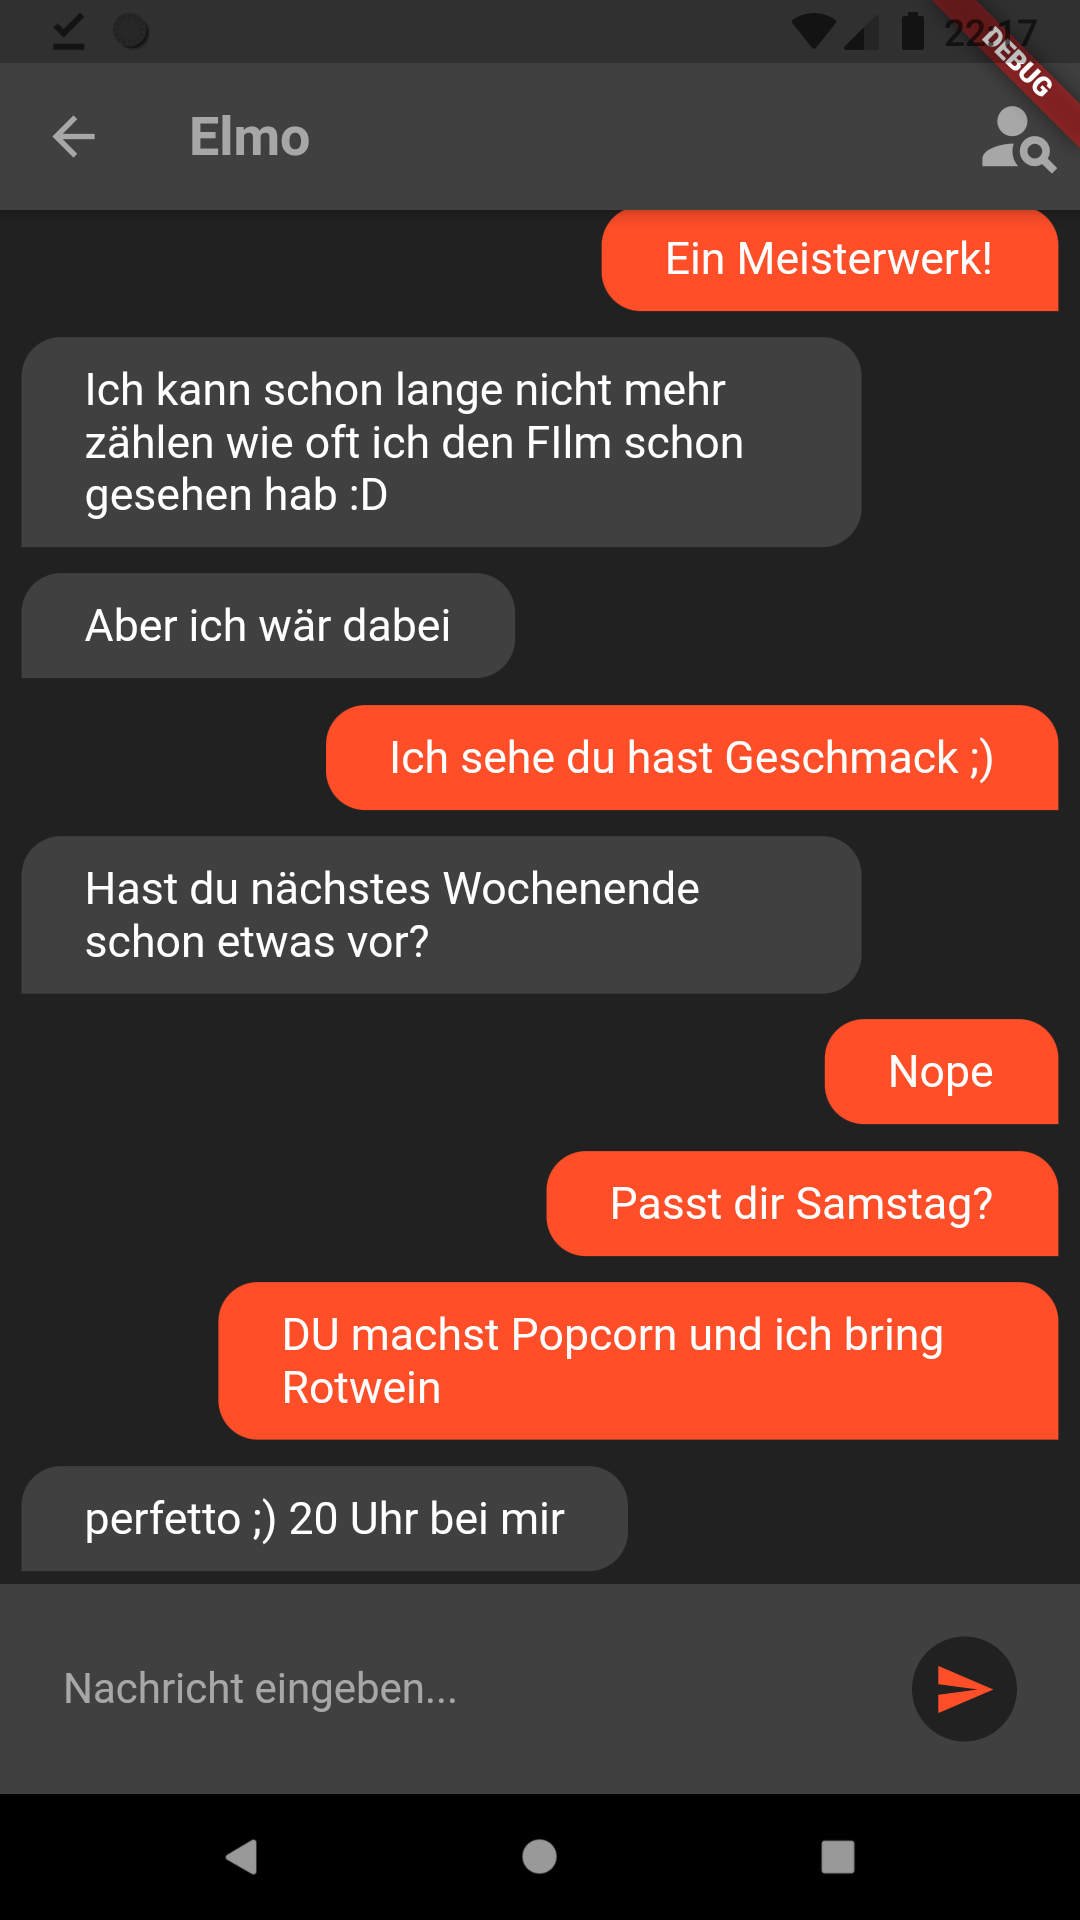
\includegraphics[scale=0.13]{Benutzeroberfläche/images/screenshot_darkmode_4.png}
	\caption{}
	\label{fig:chat_f}
	\end{subfigure}
\caption[Screenshots der Chat-Seiten]{Darstellungen und Funktionen der Chat-Screens mit (a) den aktiven Chats, (b) den Chats auf der Warteliste, (c) und (d) angenommene, bzw. abgelehnten Chats auf der Warteliste, sowie (e) einem Chatverlauf im hellen und (f) in dunklen Modus.}
\label{fig:chat_alle}
\end{figure}
